\section{Fourier 变换}

\begin{problem}{Fourier积分表示}{Fourier-Integral-Representation}
    用 Fourier 积分表示下列函数：
    \begin{enumerate}
        \item $f(x) = \begin{cases} 0, & x \leqslant 0, \\ kx, & 0 < x < T, \\ 0, & x \geqslant T; \end{cases}$
        \item $f(x) = \begin{cases} \operatorname{sgn} x, & |x| \leqslant 1, \\ 0, & |x| > 1; \end{cases}$
        \item $f(x) = \frac{1}{a^2+x^2} \quad (a > 0)$.
    \end{enumerate}
\end{problem}

\begin{solution}
    \ansitem{1}

    图形如下：
    \begin{center}
        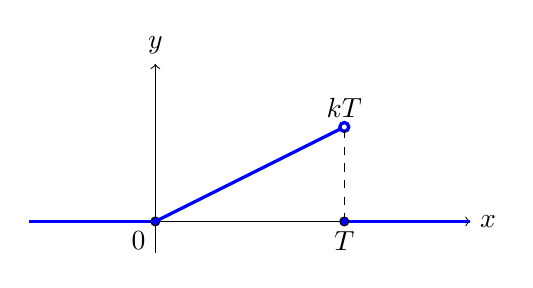
\begin{tikzpicture}[scale=0.8]
            \draw[->] (-2,0) -- (5,0) node[right] {$x$};
            \draw[->] (0,-0.5) -- (0,2.5) node[above] {$y$};
            \node[below left] at (0,0) {$0$};
            \node[below] at (3,0) {$T$};

            \draw[very thick, blue] (-2,0) -- (0,0);
            \draw[fill=blue] (0,0) circle (2pt);

            \draw[very thick, blue] (0,0) -- (3,1.5);
            \draw[fill=white, draw=blue, very thick] (3,1.5) circle (2pt);
            \node[above] at (3,1.5) {$kT$};
            \draw[dashed] (3,0) -- (3,1.5);

            \draw[very thick, blue] (3,0) -- (5,0);
            \draw[fill=blue] (3,0) circle (2pt);
        \end{tikzpicture}
    \end{center}

    函数的 Fourier 积分表示为
    \begin{equation}\label{eq:p1s1-def}
        f(x) \sim \int_{0}^{\infty} [A(\omega) \cos(\omega x) + B(\omega) \sin(\omega x)] \d\omega,
    \end{equation}
    其中，余弦系数为
    \begin{equation}\label{eq:p1s1-A}
        \begin{aligned}
            A(\omega) & = \frac{1}{\uppi} \int_{-\infty}^{\infty} f(t) \cos(\omega t) \d t                                     \\
                      & = \frac{k}{\uppi} \int_0^T t \cos(\omega t) \d t                                                       \\
                      & = \frac{k}{\uppi} \left[ \frac{T\sin(\omega T)}{\omega} + \frac{\cos(\omega T) - 1}{\omega^2} \right],
        \end{aligned}
    \end{equation}
    正弦系数为
    \begin{equation}\label{eq:p1s1-B}
        \begin{aligned}
            B(\omega) & = \frac{1}{\uppi} \int_{-\infty}^{\infty} f(t) \sin(\omega t) \d t                                  \\
                      & = \frac{k}{\uppi} \int_0^T t \sin(\omega t) \d t                                                    \\
                      & = \frac{k}{\uppi} \left[ -\frac{T\cos(\omega T)}{\omega} + \frac{\sin(\omega T)}{\omega^2} \right].
        \end{aligned}
    \end{equation}
    将\zcref{eq:p1s1-A}和\zcref{eq:p1s1-B}代入\zcref{eq:p1s1-def}，可化简得
    \begin{equation}
        \boxed{f(x) \sim \frac{k}{\uppi} \int_0^\infty \frac{T\omega\sin\omega(T-x) + \cos\omega(T-x) - \cos\omega x}{\omega^2} \d\omega}
    \end{equation}

    \ansitem{2}

    图形如下：
    \begin{center}
        \begin{tikzpicture}[scale=1.2]
            \draw[->] (-2.5,0) -- (2.5,0) node[right] {$x$};
            \draw[->] (0,-1.5) -- (0,1.5) node[above] {$y$};
            \node[below left] at (0,0) {$0$};
            \node[below] at (1,0) {$1$};
            \node[above] at (-1,0) {$-1$};

            \draw[very thick, blue] (-2.5,0) -- (-1,0);
            \draw[fill=white, draw=blue, very thick] (-1,0) circle (1.5pt);

            \draw[very thick, blue] (-1,-1) -- (0,-1);
            \draw[fill=blue] (-1,-1) circle (1.5pt);
            \draw[fill=white, draw=blue, very thick] (0,-1) circle (1.5pt);

            \draw[fill=blue] (0,0) circle (1.5pt);

            \draw[very thick, blue] (0,1) -- (1,1);
            \draw[fill=white, draw=blue, very thick] (0,1) circle (1.5pt);
            \draw[fill=blue] (1,1) circle (1.5pt);

            \draw[very thick, blue] (1,0) -- (2.5,0);
            \draw[fill=white, draw=blue, very thick] (1,0) circle (1.5pt);

            \node[left] at (0,1) {$1$};
            \node[left] at (0,-1) {$-1$};
        \end{tikzpicture}
    \end{center}

    由于 $f(x)$ 为奇函数，则 $A(\omega) = 0$．正弦系数为
    \begin{equation}\label{eq:p1s2-B}
        \begin{aligned}
            B(\omega) & = \frac{2}{\uppi} \int_{0}^{\infty} f(t) \sin(\omega t) \d t \\
                      & = \frac{2}{\uppi} \int_0^1 \sin(\omega t) \d t               \\
                      & = \frac{2(1 - \cos\omega)}{\uppi\omega}.
        \end{aligned}
    \end{equation}
    代入 Fourier 积分公式，得
    \begin{equation}
        \boxed{f(x) \sim \frac{2}{\uppi} \int_0^\infty \frac{1-\cos\omega}{\omega} \sin(\omega x) \d\omega}
    \end{equation}

    \ansitem{3}

    图形如下（以 $a=1$ 为例）：
    \begin{center}
        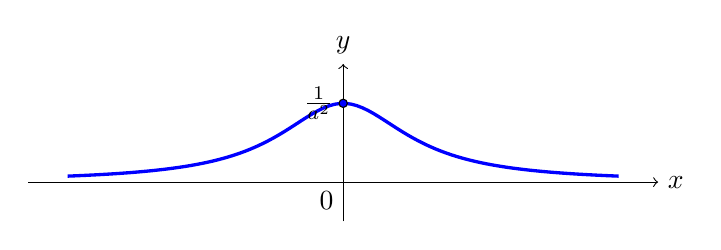
\begin{tikzpicture}[scale=1]
            \draw[->] (-4,0) -- (4,0) node[right] {$x$};
            \draw[->] (0,-0.5) -- (0,1.5) node[above] {$y$};
            \node[below left] at (0,0) {$0$};
            \draw[very thick, blue, domain=-3.5:3.5, samples=100] plot (\x, {1/(1+\x*\x)});
            \node[left] at (0,1) {$\frac{1}{a^2}$};
            \draw[fill=blue] (0,1) circle (1.5pt);
        \end{tikzpicture}
    \end{center}

    由于 $f(x)$ 为偶函数，则 $B(\omega) = 0$．余弦系数为
    \begin{equation}\label{eq:p1s3-A}
        \begin{aligned}
            A(\omega) & = \frac{2}{\uppi} \int_0^{\infty} \frac{\cos(\omega t)}{a^2+t^2} \d t \\
                      & = \frac{1}{a} \e^{-a\omega}.
        \end{aligned}
    \end{equation}
    代入 Fourier 积分公式，得
    \begin{equation}
        \boxed{f(x) \sim \frac{1}{a} \int_0^\infty \e^{-a\omega} \cos(\omega x) \d\omega}
    \end{equation}
\end{solution}

\begin{problem}{Fourier变换}{Fourier-Transform}
    求下列函数的 Fourier 变换：
    \begin{enumerate}
        \item $f(x) = x\e^{-a|x|} \quad (a > 0)$;
        \item $f(x) = \e^{-a|x|} \cos bx \quad (a > 0)$;
        \item $f(x) = \begin{cases} \cos x, & |x| \leqslant \frac{\uppi}{2}, \\ 0, & |x| > \frac{\uppi}{2}. \end{cases}$
    \end{enumerate}
\end{problem}

\begin{solution}
    \ansitem{1}

    依据定义计算其 Fourier 变换：
    \begin{equation}\label{eq:p2s1-ft}
        \begin{aligned}
            F(\omega) & = \int_{-\infty}^{\infty} x\e^{-a|x|} \e^{-\ii\omega x} \d x   \\
                      & = -\ii \int_{-\infty}^{\infty} x\e^{-a|x|} \sin(\omega x) \d x \\
                      & = -2\ii \int_0^\infty x\e^{-ax} \sin(\omega x) \d x.
        \end{aligned}
    \end{equation}
    利用分部积分法，可算得
    \begin{equation}\label{eq:p2s1-int}
        \int_0^\infty x\e^{-ax} \sin(\omega x) \d x = \frac{2a\omega}{(a^2+\omega^2)^2}.
    \end{equation}
    将\zcref{eq:p2s1-int}代入\zcref{eq:p2s1-ft}，得
    \begin{equation}
        \boxed{F(\omega) = \frac{-4\ii a\omega}{(a^2+\omega^2)^2}}
    \end{equation}

    \ansitem{2}

    已知基本变换对：
    \begin{equation}\label{eq:p2s2-basic}
        \mathcal{F}[\e^{-a|x|}] = \frac{2a}{a^2+\omega^2}.
    \end{equation}
    利用欧拉公式 $\cos bx = \frac{1}{2}\left( \e^{\ii bx} + \e^{-\ii bx} \right)$ 和频移性质，可得
    \begin{equation}\label{eq:p2s2-shift}
        \begin{aligned}
            F(\omega) & = \frac{1}{2} \left[ \mathcal{F}[\e^{-a|x|}]_{\omega \to \omega - b} + \mathcal{F}[\e^{-a|x|}]_{\omega \to \omega + b} \right] \\
                      & = \frac{a}{a^2+(\omega-b)^2} + \frac{a}{a^2+(\omega+b)^2}                                                                      \\
                      & = \frac{2a(a^2+\omega^2+b^2)}{(a^2+\omega^2+b^2)^2 - 4b^2\omega^2}.
        \end{aligned}
    \end{equation}
    因此，可得
    \begin{equation}
        \boxed{F(\omega) = \frac{2a(a^2+\omega^2+b^2)}{(a^2+\omega^2-b^2)^2 + 4a^2b^2}}
    \end{equation}

    \ansitem{3}

    依据定义计算其 Fourier 变换：
    \begin{equation}\label{eq:p2s3-ft}
        \begin{aligned}
            F(\omega) & = \int_{-\uppi/2}^{\uppi/2} \cos x \e^{-\ii\omega x} \d x    \\
                      & = 2 \int_0^{\uppi/2} \cos x \cos(\omega x) \d x              \\
                      & = \int_0^{\uppi/2} [\cos(\omega+1)x + \cos(\omega-1)x] \d x.
        \end{aligned}
    \end{equation}
    当 $\omega^2 \neq 1$ 时，积分结果为
    \begin{equation}\label{eq:p2s3-int}
        \begin{aligned}
            F(\omega) & = \left. \left[ \frac{\sin(\omega+1)x}{\omega+1} + \frac{\sin(\omega-1)x}{\omega-1} \right] \right|_0^{\uppi/2}                                         \\
                      & = \frac{\sin\left(\frac{\omega\uppi}{2} + \frac{\uppi}{2}\right)}{\omega+1} + \frac{\sin\left(\frac{\omega\uppi}{2} - \frac{\uppi}{2}\right)}{\omega-1} \\
                      & = \frac{\cos\left(\frac{\omega\uppi}{2}\right)}{\omega+1} - \frac{\cos\left(\frac{\omega\uppi}{2}\right)}{\omega-1}                                     \\
                      & = \frac{2\cos\left(\frac{\omega\uppi}{2}\right)}{1-\omega^2}.
        \end{aligned}
    \end{equation}
    当 $\omega = \pm 1$ 时，由极限或直接积分可得 $F(\pm 1) = \frac{\uppi}{2}$，这与\zcref{eq:p2s3-int}的极限值一致．因此
    \begin{equation}
        \boxed{F(\omega) = \frac{2\cos\left(\frac{\omega\uppi}{2}\right)}{1-\omega^2}}
    \end{equation}
\end{solution}

\begin{problem}{Fourier积分表示}{Fourier-Integral-Representation-Extension}
    按指定的要求将函数 $f(x) = \e^{-x} \ (0 \leqslant x < +\infty)$ 表示成 Fourier 积分．
    \begin{enumerate}
        \item 用偶延拓；
        \item 用奇延拓．
    \end{enumerate}
\end{problem}

\begin{solution}
    \ansitem{1}

    偶延拓后的函数为 $f_e(x) = \e^{-|x|}$，图形如下：
    \begin{center}
        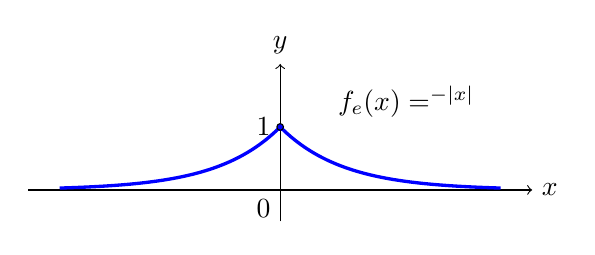
\begin{tikzpicture}[scale=0.8]
            \draw[->] (-4,0) -- (4,0) node[right] {$x$};
            \draw[->] (0,-0.5) -- (0,2) node[above] {$y$};
            \node[below left] at (0,0) {$0$};
            \draw[very thick, blue, domain=-3.5:3.5, samples=100] plot (\x, {exp(-abs(\x))});
            \node[left] at (0,1) {$1$};
            \draw[fill=blue] (0,1) circle (1.5pt);
            \node[above] at (2,1) {$f_e(x) = \e^{-|x|}$};
        \end{tikzpicture}
    \end{center}

    由于 $f_e(x)$ 为偶函数，其正弦系数 $B(\omega) = 0$．余弦系数为
    \begin{equation}
        \begin{aligned}
            A(\omega) & = \frac{2}{\uppi} \int_{0}^{\infty} \e^{-t} \cos(\omega t) \d t \\
                      & = \frac{2}{\uppi (1+\omega^2)}.
        \end{aligned}
    \end{equation}
    代入余弦型 Fourier 积分公式，得
    \begin{equation}
        \boxed{f(x) \sim \frac{2}{\uppi} \int_0^\infty \frac{\cos(\omega x)}{1+\omega^2} \d\omega}
    \end{equation}

    \ansitem{2}

    奇延拓后的函数为 $f_o(x) = \begin{cases} \e^{-x}, & x > 0, \\ 0, & x = 0, \\ -\e^x, & x < 0, \end{cases}$ 图形如下：
    \begin{center}
        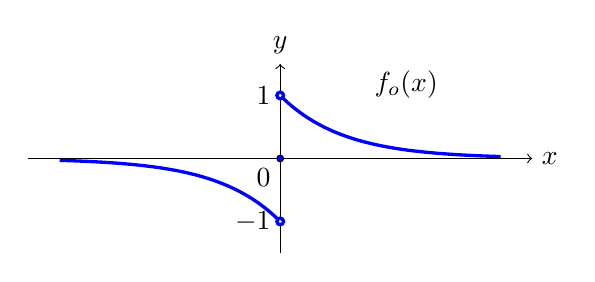
\begin{tikzpicture}[scale=0.8]
            \draw[->] (-4,0) -- (4,0) node[right] {$x$};
            \draw[->] (0,-1.5) -- (0,1.5) node[above] {$y$};
            \node[below left] at (0,0) {$0$};
            \draw[very thick, blue, domain=0.01:3.5, samples=100] plot (\x, {exp(-\x)});
            \draw[very thick, blue, domain=-3.5:-0.01, samples=100] plot (\x, {-exp(\x)});
            \draw[fill=white, draw=blue, very thick] (0,1) circle (1.5pt);
            \draw[fill=white, draw=blue, very thick] (0,-1) circle (1.5pt);
            \node[left] at (0,1) {$1$};
            \node[left] at (0,-1) {$-1$};
            \draw[fill=blue] (0,0) circle (1.5pt);
            \node[above] at (2,0.8) {$f_o(x)$};
        \end{tikzpicture}
    \end{center}

    由于 $f_o(x)$ 为奇函数，其余弦系数 $A(\omega) = 0$．正弦系数为
    \begin{equation}
        \begin{aligned}
            B(\omega) & = \frac{2}{\uppi} \int_{0}^{\infty} \e^{-t} \sin(\omega t) \d t \\
                      & = \frac{2\omega}{\uppi (1+\omega^2)}.
        \end{aligned}
    \end{equation}
    代入正弦型 Fourier 积分公式，得
    \begin{equation}
        \boxed{f(x) \sim \frac{2}{\uppi} \int_0^\infty \frac{\omega \sin(\omega x)}{1+\omega^2} \d\omega}
    \end{equation}
\end{solution}

\begin{problem}{Fourier变换与狄利克雷积分}{Fourier-Transform-Dirichlet-Integral}
    求函数 $f(x) = \begin{cases} 0, & |x| > 1, \\ 1, & |x| < 1 \end{cases}$ 的 Fourier 变换．由此证明
    \begin{equation}
        \int_{0}^{+\infty} \frac{\sin \alpha \cos \alpha x}{\alpha} \d\alpha = \begin{cases} \frac{\uppi}{2}, & |x| < 1, \\ \frac{\uppi}{4}, & |x| = 1, \\ 0, & |x| > 1. \end{cases}
    \end{equation}
\end{problem}

\begin{solution}
    函数图形如下：
    \begin{center}
        \begin{tikzpicture}[scale=1]
            \draw[->] (-3,0) -- (3,0) node[right] {$x$};
            \draw[->] (0,-0.5) -- (0,2) node[above] {$y$};
            \node[below left] at (0,0) {$0$};
            \node[below] at (1,0) {$1$};
            \node[below] at (-1,0) {$-1$};
            \draw[very thick, blue] (-3,0) -- (-1,0);
            \draw[very thick, blue] (-1,1) -- (1,1);
            \draw[very thick, blue] (1,0) -- (3,0);
            \draw[fill=white, draw=blue, very thick] (-1,0) circle (1.5pt);
            \draw[fill=white, draw=blue, very thick] (1,0) circle (1.5pt);
            \draw[fill=white, draw=blue, very thick] (-1,1) circle (1.5pt);
            \draw[fill=white, draw=blue, very thick] (1,1) circle (1.5pt);
            \node[left] at (0,1) {$1$};
        \end{tikzpicture}
    \end{center}

    首先计算 Fourier 变换：
    \begin{equation}\label{eq:ft-calc-1}
        \begin{aligned}
            F(\omega) & = \int_{-\infty}^{\infty} f(x) \e^{-\ii\omega x} \d x          \\
                      & = \int_{-1}^{1} \e^{-\ii\omega x} \d x                         \\
                      & = \left. \frac{\e^{-\ii\omega x}}{-\ii\omega} \right|_{-1}^{1} \\
                      & = \frac{2\sin\omega}{\omega}.
        \end{aligned}
    \end{equation}
    因此，可得其 Fourier 变换为
    \begin{equation}\label{eq:ft-res-2}
        \boxed{F(\omega) = \frac{2\sin\omega}{\omega}}
    \end{equation}

    根据 Fourier 逆变换公式与 Dirichlet 收敛定理，在任一点 $x$ 处有
    \begin{equation}\label{eq:inv-conv-3}
        \frac{1}{2\uppi} \int_{-\infty}^{\infty} F(\omega) \e^{\ii\omega x} \d\omega = \frac{f(x^+) + f(x^-)}{2}.
    \end{equation}
    将\zcref{eq:ft-res-2}代入\zcref{eq:inv-conv-3}中，可得
    \begin{equation}\label{eq:sub-4}
        \frac{1}{2\uppi} \int_{-\infty}^{\infty} \frac{2\sin\omega}{\omega} (\cos(\omega x) + \ii\sin(\omega x)) \d\omega = \frac{f(x^+) + f(x^-)}{2}.
    \end{equation}
    由于虚部被积函数 $\frac{\sin\omega \sin(\omega x)}{\omega}$ 关于 $\omega$ 是奇函数，在对称区间上的积分为 $0$．而实部被积函数为偶函数，故\zcref{eq:sub-4}可化简为
    \begin{equation}\label{eq:even-int-5}
        \frac{1}{\uppi} \int_{-\infty}^{\infty} \frac{\sin\omega \cos(\omega x)}{\omega} \d\omega = \frac{f(x^+) + f(x^-)}{2}.
    \end{equation}
    利用被积函数的偶性，令 $\alpha = \omega$，则有
    \begin{equation}\label{eq:alpha-int-6}
        \int_0^\infty \frac{\sin\alpha \cos(\alpha x)}{\alpha} \d\alpha = \frac{\uppi}{2} \cdot \frac{f(x^+) + f(x^-)}{2}.
    \end{equation}
    分类讨论如下：
    \begin{enumerate}
        \item 当 $|x| < 1$ 时， $f(x)$ 连续且 $f(x) = 1$， 故 $\frac{f(x^+) + f(x^-)}{2} = 1$；
        \item 当 $|x| = 1$ 时， $x = \pm 1$ 为跳跃间断点， 故 $\frac{f(x^+) + f(x^-)}{2} = \frac{1+0}{2} = \frac{1}{2}$；
        \item 当 $|x| > 1$ 时， $f(x)$ 连续且 $f(x) = 0$， 故 $\frac{f(x^+) + f(x^-)}{2} = 0$．
    \end{enumerate}
    将上述讨论代入\zcref{eq:alpha-int-6}，即证
    \begin{equation}
        \boxed{\int_{0}^{+\infty} \frac{\sin \alpha \cos \alpha x}{\alpha} \d\alpha = \begin{cases} \frac{\uppi}{2}, & |x| < 1, \\ \frac{\uppi}{4}, & |x| = 1, \\ 0, & |x| > 1. \end{cases}}
    \end{equation}
\end{solution}

\begin{problem}{Fourier逆变换}{Fourier-Inverse-Transform}
    求函数 $F(\lambda) = \lambda\e^{-\beta |\lambda|} \ (\beta > 0)$ 的 Fourier 逆变换．
\end{problem}

\begin{solution}
    函数 $F(\lambda)$ 的图形如下：
    \begin{center}
        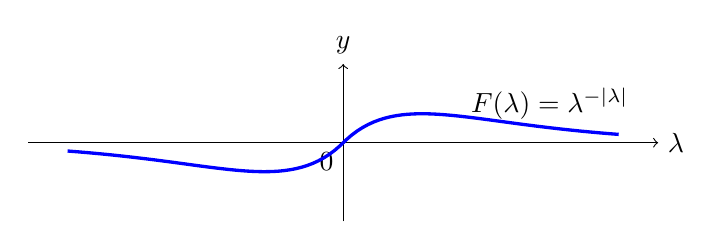
\begin{tikzpicture}[scale=1]
            \draw[->] (-4,0) -- (4,0) node[right] {$\lambda$};
            \draw[->] (0,-1) -- (0,1) node[above] {$y$};
            \node[below left] at (0,0) {$0$};
            \draw[very thick, blue, domain=-3.5:3.5, samples=100] plot (\x, {\x*exp(-abs(\x))});
            \node[right] at (1.5,0.5) {$F(\lambda) = \lambda\e^{-|\lambda|}$};
        \end{tikzpicture}
    \end{center}

    根据 Fourier 逆变换的定义，有
    \begin{equation}
        f(x) = \frac{1}{2\uppi} \int_{-\infty}^{\infty} F(\lambda) \e^{\ii\lambda x} \d\lambda.
    \end{equation}
    代入 $F(\lambda)$ 可得
    \begin{equation}\label{eq:inv-trans-def}
        \begin{aligned}
            f(x) & = \frac{1}{2\uppi} \int_{-\infty}^{\infty} \lambda \e^{-\beta|\lambda|} (\cos(\lambda x) + \ii \sin(\lambda x)) \d\lambda \\
                 & = \frac{\ii}{\uppi} \int_{0}^{\infty} \lambda \e^{-\beta\lambda} \sin(\lambda x) \d\lambda.
        \end{aligned}
    \end{equation}
    利用拉普拉斯积分性质，有
    \begin{equation}
        \int_0^\infty \e^{-\beta\lambda} \sin(\lambda x) \d\lambda = \frac{x}{\beta^2+x^2}.
    \end{equation}
    对上式关于参数 $\beta$ 求导，可得
    \begin{equation}
        -\int_0^\infty \lambda \e^{-\beta\lambda} \sin(\lambda x) \d\lambda = -\frac{2\beta x}{(\beta^2+x^2)^2}.
    \end{equation}
    即
    \begin{equation}\label{eq:int-formula-sin}
        \int_0^\infty \lambda \e^{-\beta\lambda} \sin(\lambda x) \d\lambda = \frac{2\beta x}{(\beta^2+x^2)^2}.
    \end{equation}
    将\zcref{eq:int-formula-sin}代入\zcref{eq:inv-trans-def}，可得
    \begin{equation}
        \boxed{f(x) = \frac{2\ii\beta x}{\uppi(\beta^2 + x^2)^2}}
    \end{equation}
\end{solution}

\endinput
